% Misc. Definitions
%% Color definitions
\definecolor{Fgreen}{RGB}{34,139,34}


%--------------------------------------------------
% Introduction
%--------------------------------------------------
%--------------------------------------------------

%DEFINE BASE PROBLEM, AND DISCUSS WHAT WE MEAN BY "LOCAL MEASUREMENTS"!!!\\

%Angular synchronization refers to the problem of recovering $d$ angles
%$\phi_1, \phi_2, \dots, \phi_d \in [0, 2\pi)$ given noisy and possibly
%    incomplete difference measurements of the form
%%
%\[  \phi_{ij} := \phi_i - \phi_j, \qquad (i,j) \in 
%        \{1,2,\dots,d\} \times \{1,2,\ldots,d\}. \]
%%
%This problem has important applications in network delay analysis
%\cite{network_ref}, optics \cite{optics_ref} and computer vision
%\cite{cvision_ref}. In this paper, however, we are interested in angular
%synchronization problems that arise when performing {\em phase
%retrieval} from {\em local correlation} measurements. 

Consider the problem of recovering a vector $\x_0 \in \C^d$ from measurements $\y \in \R^D$ with entries $y_j$ given by
\begin{equation}
y_j = |\langle \mathbf{a}_j, \x_0 \rangle|^2 + \eta_j, \quad\quad j = 1,\ldots, D.\label{eq:phase_ret}
\end{equation}
Here the measurement vectors $\mathbf{a}_j\in \C^d$ are known and the scalars $\eta_j \in \R$ denote noise terms.  This problem is known as the \emph{phase retrieval problem} (see, e.g., \cite{millane1990phase, walther1963question}), as we may think of the $|\cdot|^2$ in \eqref{eq:phase_ret} as erasing the phases of the measurements $\langle \a_j, \x_0 \rangle$ in an otherwise linear system of equations.
%% Had the phase of $\langle \a_j, \x \rangle$ not been erased in \eqref{eq:phase_ret}, inverting the map from $\C^d$ to $\R^D$ induced by \eqref{eq:phase_ret}  corresponds to solving a linear system had the phase of $\langle \a_j, \x \rangle$ not been erased, 

The phase retrieval problem  arises in many important signal acquisition schemes, including crystallography and ptychography (e.g., \cite{millane1990phase%, Rudenberg2008
}, see Figure \ref{fig:ptychography_setup}), diffraction imaging \cite{gerchberg1972practical}, and optics \cite{millane1990phase, walther1963question}, %, and array imaging \cite{chai2011array}
  among many others.  Due to the breadth and importance of the applications, there has been significant interest in developing efficient algorithms to solve this problem. Indeed, one of the first algorithms proposed came in the early 1970's with the work of Gerchberg and Saxton \cite{gerchberg1972practical}. Since then many variations of their method have been proposed (e.g, \cite{bauschke2003hybrid,bauschke2002phase,elser2003phase,fienup1978reconstruction,takajo1997numerical,takajo1999further,takajo1998study}) and used widely in practice.  On the other hand -- until recently -- there have not been theoretical guarantees concerning the conditions under which these algorithms recover the underlying signal and the extent to which they can tolerate measurement error. Nevertheless, starting in 2006 a growing body of work (e.g., \cite{ balan2007fast, balan2006signal, bandeira2013near, bodmann2013stable, candes2012phaselift, eldar2012phase, IVW2015_FastPhase, li2012sparse}) has emerged, proposing new methods with theoretical performance guarantees under various assumptions on the signal $\x_0$ and the measurement vectors $\a_j$. Unfortunately, the assumptions (especially on the measurement vectors) often do not correspond to the setups used in practice. In particular, the mathematical analysis often requires that the measurement vectors be random or generic (e.g., \cite{balan2006signal, bandeira2013near, candes2012phaselift}) while in practice the measurement vectors are a deterministic aspect of the imaging apparatuses employed.  A main contribution of this paper is analyzing a construction that more closely matches practicable and deterministic measurement schemes. We propose a two-stage algorithm for solving the phase retrieval problem in this setting and we analyze our method, providing upper bounds on the associated reconstruction error. 

In short, we provide theoretical error guarantees for a numerically efficient reconstruction algorithm in a measurement setting that closely resembles measurements used in practice. 


\subsection{Local Correlation Measurements}
\label{sec:locCorrMeas}

Consider the case where the vectors $\a_j$ represent shifts of compactly-supported vectors $\m_j, j = 1, \ldots, K$ for some $K \in \N$.  Using the notation $[n]_k:=\{k,\ldots,k+n-1\}\subset \N$, and defining $[n]:=[n]_1$ we take $\x_0, \m_j \in \C^d$ with $\supp(\m_j)\subset[\delta]\subset [d]$ for some $\delta \in \N$.  We also denote the space of Hermitian matrices in $\C^{k \times k}$ by $\H^k$.  Now we have measurements of the form \begin{equation} (\y_\ell)_j = |\langle \x_0, S^*_\ell \m_j \rangle|^2, \quad (j, \ell) \in [K] \times P, \label{eq:shift_model} \end{equation} where $P \subset [d]_0$ is arbitrary and $S_\ell : \C^d \to \C^d$ is the discrete circular shift operator, namely \begin{equation*} (S_\ell \x_0)_j = (\x_0)_{\ell + j}. \end{equation*}  One can see that \eqref{eq:shift_model} represents the modulus squared of the correlation between $\x_0$ and locally supported measurement vectors.  Therefore, we refer to the entries of $\y$ as local correlation measurements.
%
%
Following \cite{balan2006signal,candes2012phaselift,IVW2015_FastPhase}, the problem may be lifted to a linear system on the space of $\C^{d \times d}$ matrices.  In particular, we observe that 
\begin{align*}
	(\y_\ell)_j &= |\langle S_\ell \x_0, \m_j\rangle|^2 = \m_j^* (S_\ell \x_0) (S_\ell \x_0)^* \m_j \\
	&= \langle \x_0 \x_0^*, S_\ell^* \m_j \m_j^* S_\ell\rangle,
\end{align*}
where the inner product above is the Hilbert-Schmidt inner product. Restricting to the case $P = [d]_0$,  for every matrix $A \in \Span\{S_\ell^* \m_j \m_j^* S_\ell\}_{\ell, j}$ we have $A_{ij} = 0$ whenever $|i - j| \mod d \ge \delta$.  Therefore, we introduce the family of operators $T_k : \C^{d \times d} \to \C^{d \times d}$ given by \begin{equation} T_k(A)_{ij} = \left\{\begin{array}{r@{,\qquad}l} A_{ij} & |i - j| \mod d < k \\ 0 & \text{otherwise}. \end{array}\right. \label{eq:T_delta} \end{equation}  Note that $T_\delta$ is simply the orthogonal projection operator onto its range $T_\delta(\C^{d \times d}) \supseteq \Span\{S_\ell^* \m_j \m_j^* S_\ell\}_{\ell, j}$; therefore, \begin{equation} (\y_\ell)_j = \langle \x_0 \x_0^*, S_\ell^* \m_j \m_j^* S_\ell \rangle = \langle T_{\delta}(\x_0 \x_0^*), S_\ell^* \m_j \m_j^* S_\ell \rangle, \quad (j, \ell) \in [K] \times P. \label{eq:lifted_system} \end{equation}  

For convenience, we set $D := K|P|$ and define the map $\mathcal{A} : \C^{d \times d} \to \C^D$ 
\begin{equation}\mathcal{A}(X) = [\langle X, S_\ell^* \m_j \m_j^* S_\ell \rangle]_{(\ell, j)}.\label{eq:linear}\end{equation}  
Sometimes, we consider $\mathcal{A}|_{T_{\delta}(\C^{d \times d})}$, the restriction of $\mathcal{A}$ to the domain $T_{\delta}(\C^{d \times d})$; indeed, if this linear system is injective on $T_\delta(\C^{d \times d})$, then we can readily solve for 
\begin{equation}T_\delta(\x_0 \x_0^*) =: X_0 \label{equdef:X0} \end{equation}  
using our measurements $(\y_\ell)_j = (\mathcal{A}(\x_0 \x_0^*))_{(\ell,j)}$.
In \cite{IVW2015_FastPhase}, deterministic masks $\m_j$ were constructed for which \eqref{eq:lifted_system} was indeed invertible for certain choices of $K$ and $P$.  An additional construction is given below in \S\ref{sec:MeasMatrix}.

Improving on \cite{IVW2015_FastPhase}, we can further see that $\x_0$ can be deduced from $X_0$ up to a global phase in the noiseless case as follows:  First, $X_0$ immediately gives the magnitudes of the entries of $\x_0$ since $(X_0)_{ii} = |(x_0)_i|^2$.  
The only challenge remaining, therefore, is to find $\arg((x_0)_i)$ up to a global phase.  We proceed by defining $\tilde{\x}_0$ and $\widetilde{X}_0$ by \[(\tilde{x}_0)_i = \sgn((x_0)_i)\] \[(\widetilde{X}_0)_{ij} = \left\{\begin{array}{r@{,\quad}l} \sgn((X_0)_{ij}) & |i - j| \mod d < \delta \\ 0 & \text{otherwise} \end{array}\right.,\] where $\sgn : \C \to \C$ is the usual normalization mapping \[\sgn(z) = \left\{\begin{array}{r@{,\qquad}l} \dfrac{z}{|z|} & z \neq 0 \\ 1 & \text{otherwise} \end{array}\right..\]  We emphasize that 
\begin{equation}
\tX_0= \frac{X_0}{|X_0|}= \frac{T_\delta(\x_0\x_0^*)}{|T_\delta(\x_0\x_0^*)|} \ \text{and} \ \widetilde{\x}_0 = \frac{\x_0}{|\x_0|},
\label{eq:X_0} 
\end{equation} 
where the divisions are taken component-wise.  Indeed, in \cite{IV_SPIE}, it was shown that the phases of the entries of $\x_0$ (up to a global phase) are given by the leading eigenvector of $\widetilde X_0$.  Moreover, it was shown that this leading eigenvector is unique.  Lemma \ref{lem:EigGap} of this paper improves in these results by giving a lower bound on the gap between the top two eigenvalues of $\widetilde X_0$.  This better understanding of the spectrum of $\widetilde X_0$ is then leveraged to analyze the robustness of this eigenvector-based phase retrieval method to measurement noise.

%The robustness of this eigenvector method to noise and the associated recovery guarantees for the phase retrieval problem are the primary subject of this paper.% \RSnote{ we should comment on the speed of that method.}

%% \RSnote{Need to say something here about what we do in this paper, and connect this with the previous paragraph as well as the next load of stuff on ptychography.}

%Phase retrieval \cite{balan2006signal,shechtman2015phase} arises naturally in a wide range of important practical applications ranging from 
%molecular imaging modalities such as X-Ray crystallography and
%Ptychography \cite{Rodenburg2008}, where the underlying physics dictates
%that we can only acquire (squared) magnitude or phaseless measurements.
%As one may imagine, this is an extremely challenging
%mathematical problem even in the setting when the measurements are noise-free as the phase encapsulates a significant amount of
%structure in the underlying signal. %hence, recovering the signal from phaseless data is a non-trivial task. 
%To complicate things further, often the physics associated with the problem constrains the type of measurements one acquires. 

%--------------------------------------------------
% Main Result 
%--------------------------------------------------
\subsection{Contributions}
\label{sec:mainRes}

In this paper, we analyze a phase retrieval algorithm (Algorithm \ref{alg:phaseRetrieval1}) for estimating a vector $\x_0$ from noisy localized measurements of the form
 \begin{equation} (\y_\ell)_j = |\langle \x_0, S^*_\ell \m_j \rangle|^2 + n_{j \ell}, \quad (j, \ell) \in [2\delta-1] \times [d]_0 \label{eq:shift_model_noise}.\end{equation}
%which was originally proposed in \cite{IV_SPIE}.
 This algorithm is composed of two main stages. First, we apply the inverse of the linear operator
$$\mathcal{A}|_{T_{\delta}(\C^{d \times d})}: T_{\delta}(\C^{d\times d}) \to \C^{(2\delta-1)d}$$
  %$\mathcal{A}|_{T_{\delta}(\C^{d \times d})}$, 
  defined immediately after \eqref{eq:linear}, to obtain a Hermitian estimate ${X}$ of $T_\delta{(\x_0\x_0^*)}$ given by 
  \begin{equation}X = \Big( (\mathcal{A}|_{T_\delta(\C^{d\times d})})^{-1} {\bf y}\Big)/2 + \Big( (\mathcal{A}|_{T_\delta(\C^{d\times d})})^{-1} {\bf y}\Big)^*/2  \in T_\delta(\C^{d\times d}) \label{eq:X}
  .\end{equation} In particular, our choice of $\m_j$ as described in Section \ref{sec:MeasMatrix} ensures that $\mathcal{A}|_{T_{\delta}(\C^{d \times d})}$ is both invertible and well conditioned. Next, once we have an approximation of $T_\delta(\x_0 \x_0^*)$, we estimate the magnitudes and phases of the entries of $\x_0$ separately. 
  
  For the magnitudes, we simply use the square-roots of the diagonal entries of $X$. For the phases, we use the normalized eigenvector corresponding to the top eigenvalue of \begin{equation}\widetilde{X}:=\frac{X}{|X|},\label{eq:Xtilde}\end{equation}
where the operations are considered element-wise.  The hope is that the leading eigenvector of $\tX$ will serve as a good approximation to the leading eigenvector of $\tX_0$, which is seen in Section \ref{sec:Spectrum} (see also \cite{IV_SPIE}) to indeed be a scaled version of the phase vector $\tx_0$ (up to a global phase ambiguity).  The entire method is summarized in Algorithm \ref{alg:phaseRetrieval1}, and its associated recovery guarantees are presented in Theorem \ref{Prop:RecovRes}, while its computational complexity is discussed after the theorem in \S\ref{sec:RuntimeAlg1}.  Here and throughout the paper, $\ee = 2.71828\ldots$ refers to the base of the natural logarithm and $\ii$ refers to the imaginary unit.
\begin{algorithm}
\renewcommand{\algorithmicrequire}{\textbf{Input:}}
\renewcommand{\algorithmicensure}{\textbf{Output:}}
\caption{Fast Phase Retrieval from Local Correlation Measurements}
\label{alg:phaseRetrieval1}
\begin{algorithmic}[1]
    \REQUIRE Measurements $\y\in \R^D$ as per \eqref{eq:shift_model_noise}
    \ENSURE ${\bf x} \in \mathbbm{C}^d$ with ${\bf x} \approx \mathbbm{e}^{-\mathbbm{i} \theta} {\bf x}_0$ for some $\theta \in [0, 2 \pi]$
    \STATE Compute the Hermitian matrix $X = \Big( (\mathcal{A}|_{T_\delta(\C^{d\times d})})^{-1} {\bf y}\Big)/2 + \Big( (\mathcal{A}|_{T_\delta(\C^{d\times d})})^{-1} {\bf y}\Big)^*/2  \in T_\delta(\C^{d\times d})$ as an estimate of $T_\delta(\x_0\x_0^*)$%(see \eqref{equ:LinProb}) %--[??? use ${\bf z}' = W (M')^{-1} P {\bf y}$ instead -- see \eqref{def:Wdef}) ?]
    \STATE Form the banded matrix of phases, $\tilde{\X} \in T_\delta(\mathbbm{C}^{d \times d})$, by normalizing the non-zero entries of $\X$ %(replacing any zero entries in the band with $1$'s)
    \STATE Compute the top eigenvector $u \in \C^d$ of $\tilde{\X}$ and set $\tx := \sgn(u)$.
    \STATE Set $x_j = \sqrt{X_{j,j}} \cdot (\tilde{x})_j$ for all $j \in [d]$ to form $\x \in \mathbbm{C}^d$
    %\STATE Set $\x = W^* \tilde{\x}$ 
    \end{algorithmic}
\end{algorithm}


\begin{theorem}
Suppose $\delta > 2$ and $d \ge 4 \delta$.  Let $(x_0)_{\rm min} := \min_j |(x_0)_j|$ be the smallest magnitude of any entry in $\x_0 \in \mathbbm{C}^d$.  Then, the estimate $\x$ produced in Algorithm~\ref{alg:phaseRetrieval1} satisfies 
\[ \min_{\theta \in [0, 2 \pi]} \left\Vert  \x_0 - \mathbbm{e}^{\mathbbm{i} \theta} \x \right\Vert_2 \leq C \left( \frac{\Vert \x_0 
        \Vert_{\infty}}{(x_0)^2_{\rm min}} \right) \left( \frac{d}{\delta} \right)^2 \kappa \| \n \|_2 + C d^{\frac{1}{4}} \sqrt{\kappa \| \n \|_2 },\]
where $\kappa > 0$ is the condition number of the system \eqref{eq:X} and $C \in \mathbb{R}^+$ is an absolute universal constant.
\label{Prop:RecovRes}
\end{theorem}

Theorem~\ref{Prop:RecovRes}, which deterministically depends on both the masks and the signal, provides improvements over the first deterministic theoretical robust recovery guarantees proven in \cite{IVW2015_FastPhase} for a wide class of non-vanishing signals.  Momentarily consider, e.g., the class of ``flat'' vectors $\x_0 \in \mathbbm{C}^d$ for which both $(i)$ $(x_0)_{\rm min} \geq \frac{\| \x_0 \|_2}{2 \sqrt{d}}$, and $(ii)$ $\left( \frac{\Vert \x_0 \Vert_{\infty}}{(x_0)^2_{\rm min}} \right) \leq \tilde{C}$ for some absolute constant $\tilde{C} \in \mathbbm{R}^+$, hold.  The main deterministic result of \cite{IVW2015_FastPhase} also applies to this class of vectors and states that an algorithm exists which can achieve the following robust recovery guarantee.

\begin{theorem}[See Theorem 5 in \cite{IVW2015_FastPhase}]
There exist fixed universal constants $C,C' \in \mathbbm{R}^+$ such that the following holds for all $\x_0 \in \mathbbm{C}^d$ of the class mentioned above:  Let 
$\| \x_0 \|_2 \geq C d  \sqrt{\left(\delta - 1 \right)\| \n \|_2}$.  Then, the  algorithm in \cite{IVW2015_FastPhase}, when provided with noisy measurements of $\x_0 \in \mathbbm{C}^d$ \eqref{eq:shift_model_noise} resulting from the masks discussed in Example 1 of \S\ref{sec:MeasMatrix}, will output a vector  $\x \in \mathbbm{C}^d$ satisfying
\[ \min_{\theta \in [0, 2 \pi]} \left\Vert  \x_0 - \mathbbm{e}^{\mathbbm{i} \theta} \x \right\Vert_2 \leq C' d  \sqrt{\left(\delta - 1 \right)\| \n \|_2 }.\]
\label{Thm:OLDRecovRes}
\end{theorem}

Comparing the error bounds provided by Theorems~\ref{Prop:RecovRes} and~\ref{Thm:OLDRecovRes} for the class of flat vectors $\x_0$ mentioned above when using measurements resulting from the masks discussed in Example 1 of \S\ref{sec:MeasMatrix},\footnote{Note that the condition number $\kappa$ mentioned in Theorem~\ref{Prop:RecovRes} for the masks discussed in Example 1 of \S\ref{sec:MeasMatrix} is $\mathcal{O}(\delta^2)$.  See Theorem~\ref{thm:WellCondMeas} below for a more exact statement.  All asymptotic notation is with respect to $d \rightarrow \infty$.  Below $\delta$ is always assumed to be independent of (and less than) $d$ unless otherwise noted.} we can see that  Theorem~\ref{Prop:RecovRes} makes the following improvements over Theorem~\ref{Thm:OLDRecovRes}:
\begin{itemize}
\item Theorem~\ref{Prop:RecovRes} improves on the error bound of Theorem~\ref{Thm:OLDRecovRes} for arbitrary small-norm noise $\n$ having $\| \n \|_2 = \mathcal{O} \left( \delta / d^2 \right).$
\item Theorem~\ref{Thm:OLDRecovRes}'s error bound breaks down entirely for noise $\n$ with $\ell^2$-norm on the order of $\| \n \|_2 = \Theta \left( \frac{\| \x_0 \|^2_2}{\delta d^2} \right)$.   Theorem~\ref{Prop:RecovRes}'s error bound, on the other hand, still provides non-trivial error guarantees for such noise levels as long as $\| \x_0 \|_2 = \mathcal{O}\left( \delta \right)$.\footnote{This allows Theorem~\ref{Prop:RecovRes} to cover, e.g., the case of larger $\delta = \Omega \left( \sqrt{d} \right)$.}
\end{itemize}
In addition, Theorem~\ref{Prop:RecovRes} also applies to a more general set of masks and a larger class of signals $\x_0$ than Theorem~\ref{Thm:OLDRecovRes} does.  And, perhaps most importantly, Algorithm~\ref{alg:phaseRetrieval1} generally outperforms the algorithm referred to by Theorem~\ref{Thm:OLDRecovRes} numerically for all noise levels (see, e.g., Figures~\ref{fig:eig_vs_greedy} and~\ref{fig:global_vs_local_ptych} in \S\ref{sec:NumEval}).  Theorem~\ref{Prop:RecovRes} provides theoretical error guarantees for this numerically improved method.

We note that the  $\mathcal{O}\left( \left(\frac{d}{\delta} \right)^2 \right)$-factor in the first term of the error bound provided by Theorem~\ref{Prop:RecovRes} is probably suboptimal, especially in practice.  Indeed, Theorem~\ref{Prop:RecovRes} provides a worst-case error guarantee that holds for any arbitrary (including worst-case/adversarial) perturbation $\n$ of the measurements \eqref{eq:shift_model_noise}.  %The fact that this $ \left(d / \delta \right)^2$-factor is \textit{quadratic} in $d/\delta$ in Theorem~\ref{Prop:RecovRes} is probably due to Theorem~\ref{Prop:RecovRes} being suboptimal. 
However, while the quadratic dependence on $d/\delta$ is probably suboptimal, \textit{some} dependence on $d/\delta$ likely exists for worst-case additive-noise in our local measurement setting.  There is, e.g., numerical evidence that the empirical noise robustness of many phase retrieval methods deteriorates as $d$ grows for local measurements whose support size $\delta$ is held fixed.  We will leave a rigorous theoretical investigation of the optimal scaling of such noise robustness guarantees with $d/\delta$ to future work.  For the time being we will simply note here that the $\mathcal{O}\left( \left(\frac{d}{\delta} \right)^2 \right)$-factor %in the first term of the error bound provided by Theorem~\ref{Prop:RecovRes} 
is mainly a product of the relatively small eigenvalue gap of the matrix $\tX_0$ defined in \eqref{eq:X_0} above.  See \S\ref{sec:Spectrum} below for more details.

\subsection{The Runtime Complexity of Algorithm~\ref{alg:phaseRetrieval1}}
\label{sec:RuntimeAlg1}

Consider now the computational complexity of Algorithm~\ref{alg:phaseRetrieval1} (assuming, of course, that $\mathcal{A}|_{T_\delta(\C^{d\times d})}$ is actually invertible).  One can see that line 1 can  always be done in at most $\mathcal{O}(d \cdot \delta^3 + \delta \cdot d \log d)$ flops using a block circulant matrix factorization approach (see Section 3.1 in \cite{IVW2015_FastPhase}). In certain cases one can improve on this; for example, the second (new) mask construction of Section \ref{sec:MeasMatrix} allows line 1 to be performed in only $\mathcal{O}(d\cdot\delta)$ flops.  Even in the worst case, however, if one precomputes this block circulant matrix factorization in advance given the masks $\m_j$ then line 1 can always be done in $\mathcal{O}(d \cdot \delta^2 + \delta \cdot d \log d)$ flops thereafter.  

The top eigenvector $\tilde{\x}$ of $\tilde{X}$ is guaranteed to be found in line 3 of Algorithm~\ref{alg:phaseRetrieval1} in the low-noise (e.g., noiseless) setting via the shifted inverse power method with shift $\mu := 2 \delta - 1$ and initial vector ${\bf e}_1$ (the first standard basis vector).  
More generally, one may utilize the Rayleigh quotient iteration with the initial eigenvalue estimate fixed to $2 \delta - 1$ for the first few iterations.
In either case, each iteration can be accomplished with $\mathcal{O}(d \cdot \delta^2)$ flops due to the banded structure of $\tilde{X}$ (see, e.g., \cite{trefethen1997numerical}).  In the low-noise setting the top eigenvector $\tilde{\x}$ can be computed to machine precision in $\mathcal{O}(\log d)$ such iterations,\footnote{To see why $\mathcal{O}(\log d)$ iterations suffice one can appeal to lemmas~\ref{lem:spectrum}~and~\ref{lem:EigGap} below.  Let $|\lambda_1| > |\lambda_2| \geq \dots \geq |\lambda_d|$ be the eigenvalues of $\tilde{X}$ with associated orthonormal eigenvectors ${\bf u}_j \in \mathbbm{C}^d$.  Let $\delta := |\lambda_1| - |\lambda_2| > 0$.  When the noise level is sufficiently low (so that $\tilde{X} \approx \tilde{X}_0$) one will have both $(i)$ $|{\bf e}^*_1 {\bf u}_j| = \Theta(1/\sqrt{d})~\forall j \in [d]$, and $(ii)$ $\mu \in (\lambda_1-\delta/4, \lambda_1+\delta/4)$ be true.  Thus, we will have that there exists some unit norm ${\bf r} \in \mathbbm{C}^d$ such that
$$\frac{\left( \tilde{X} - \mu I \right)^{-k}{\bf e}_1}{\left\| \left( \tilde{X} - \mu I \right)^{-k}{\bf e}_1 \right\|_2} = \frac{{\bf u}_1 + \sum^d_{j=2} \mathcal{O}\left( \left|\frac{\lambda_1 - \mu}{\lambda_j - \mu} \right|^k \right) {\bf u}_j}{1 + \mathcal{O}\left( \frac{d}{9^k} \right)} = {\bf u}_1 + \mathcal{O} \left( \frac{d}{3^k} \right) {\bf r}$$ holds for any given integer $k = \Omega \left( \log_3 d \right)$.} 
for a total flop count of $\mathcal{O}(\delta^2 \cdot d \log d)$ for line 3 in that case.  In total, then, one can see that Algorithm~\ref{alg:phaseRetrieval1} will always require just $\mathcal{O}(\delta^2 \cdot d \log d + d \cdot \delta^3)$ total flops in low-noise settings.  Furthermore, in all such settings a measurement mask support of size $\delta = \mathcal{O}(\log d)$ appears to suffice.

\subsection{Connection to Ptychography}
\label{sec:conn_pty}

\begin{figure}[hbtp]
    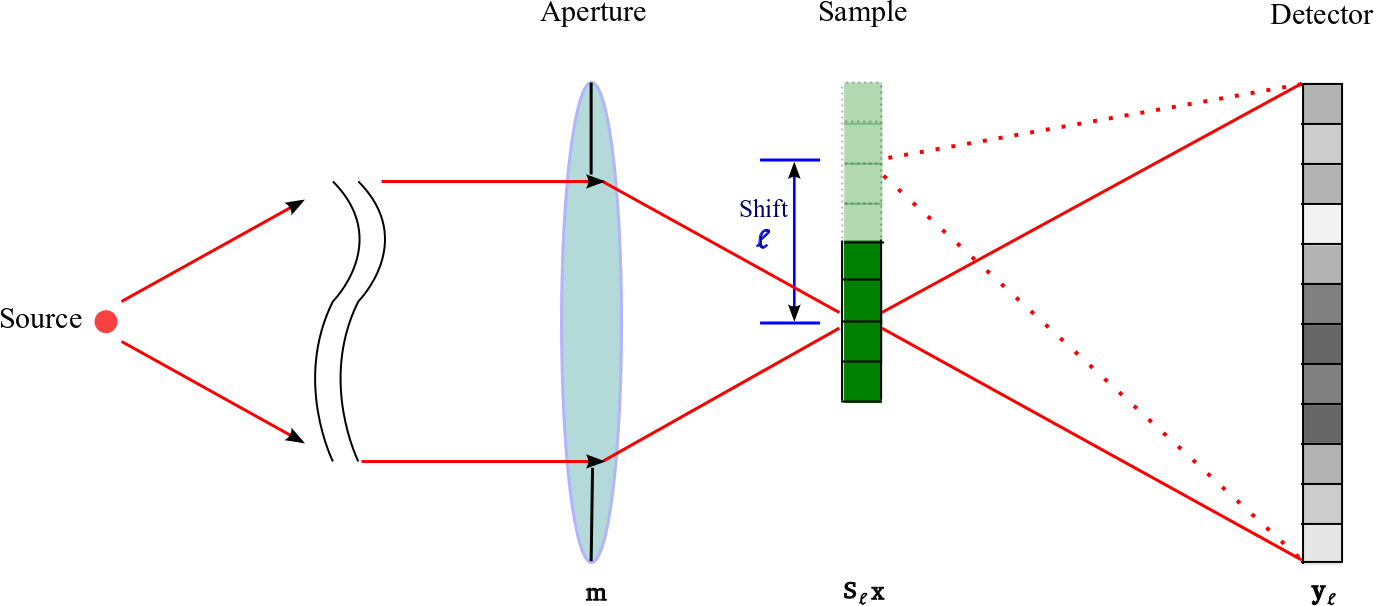
\includegraphics[scale=0.25]{pics/ptych1D}
    \caption{Illustration of one-dimensional ptychographic imaging {\small 
        (Adapted from ``Fly-scan ptychography'', Huang et al., 
        Scientific Reports 5 (9074), 2015.)} }
    \label{fig:ptychography_setup}
\end{figure}

In ptychographic imaging (see Fig.
\ref{fig:ptychography_setup}), small regions of a specimen are
illuminated one at a time and an intensity\footnote{By intensity,
we mean magnitude squared.} detector captures each of the
resulting  diffraction patterns. Thus each of the ptychographic
measurements is a local measurement, which under certain
assumptions (e.g., appropriate wavelength of incident radiation,
far-field Fraunhofer approximation), can be modeled as
\cite{Dierolf2008Ptych,Goodman2005IntroFourierOptics}%\RSnote{We need some citations here to justify this model}
%
\begin{equation}
    y(t, \omega) = \left \vert \mathcal F [ \widetilde h \cdot S_t f ] (\omega) 
       \right \vert^2 + \eta(t, \omega) .\label{eq:ptych}
\end{equation} 
%we acquire a sequence of possibly noisy, {\em local} (as
%opposed to {\em global}) snapshots of the magnitude of the underlying specimen. %The need
%to minimize the number of measurements acquired and inevitable
%measurement errors in the imaging process only accentuate the complexity
%of this phase retrieval problem.
%
%
%To set the stage for the discussion in this paper, consider the
%one-dimensional ptychographic imaging setup in Fig.~
%\ref{fig:ptychography_setup}, w
%Specifically, in the one-dimensional ptychography setting we focus on, . Under certain conditions (appropriate wavelength of
%incident radiation, far-field Fresnel approximation), it is possible to
%show \cite{?} that the acquired magnitude measurements of the form 
%%
%\begin{equation*}
%    y_\ell = \left \vert \mathcal F [ \widetilde m \circ S_\ell x ]
%       \right \vert^2,
%\end{equation*}
%%
Here, $\mathcal F$ denotes the Fourier transform, $f : [0, 1] \to \C$ represents
the unknown test specimen, $S_t$ is the shift operator defined
via $$(S_t f)(s) := f(s + t),$$ and $\widetilde h : [0, 1] \to \C$ is the so-called
illumination function %\RSnote{Aditya, is this standard terminology?} 
\cite{arXiv:1105.5628_MarchesiniEtAl}
of the imaging system. %Note that squaring the magnitude of the Fourier transform above means that $y_\ell$ is a
%phaseless diffraction measurement corresponding to a specific
%shift (by $\ell$) of the test specimen.  
To account for the local nature of the measurements in
\eqref{eq:ptych}, we assume that $\text{supp}(\widetilde h)
\subset \text{supp} (f)$.

As the phase retrieval problem is inherently non-linear and requires sophisticated computer algorithms to solve, consider the discrete version of \eqref{eq:ptych}, with $\widetilde{\m}, \x_0 \in \C^d$ discretizing $\widetilde{h}$ and $f$.  Thus \eqref{eq:ptych}, in the absence of noise, becomes 
%
\begin{equation}
    (\y_\ell)_j = \left \vert \sum_{n=1}^d \widetilde m_n \, (x_0)_{n+\ell} \,
      \mathbbm e^{-\frac{2\pi \mathbbm i (j-1) (n-1)}d} 
      \right \vert^2, \quad (j,\ell) \in [d] \times  
      [d]_0, 
  \label{eq:1d_ptycho}
\end{equation}
%
where indexing is
considered modulo-$d$, so $(\y_\ell)_j$
is a diffraction measurement corresponding to the $j^{th}$ Fourier mode
of a circular $\ell$-shift of the specimen. We use circular shifts for convenience and we remark that this is appropriate as one can zero-pad $\x_0$ and $\widetilde{\m}$  in \eqref{eq:1d_ptycho} and obtain the same $(\y_\ell)_j$ as one would with non-circular shifts. In practice, one may not need to use all the shifts $\ell \in [d]_0$ as a subset may suffice.  Defining $\m_j \in \C^d$ by \begin{equation} (\m_j)_n = \overline{\widetilde m_n} \, \mathbbm e^{\frac{2\pi \mathbbm i (j-1) (n-1)}d} \label{eq:ptychm} \end{equation} and rearranging \eqref{eq:1d_ptycho}, we obtain
\begin{align}
    (\y_\ell)_j &= \left \vert \sum_{n=1}^d (x_0)_{n+\ell} \, \overline{(\m_j)_n} \right \vert^2 \label{eq:loco_measurements} %\\ 
        %&
        = \left \vert \sum_{n=1}^\delta (x_0)_{n+\ell} \, \overline{(\m_j)_n} \right \vert^2 \\
        &= \lvert \langle S_\ell \x_0, \m_j \rangle \rvert^2 \notag %\\
       % &
       = \langle S_\ell \x_0 \x_0^* S_\ell^*, \m_j \m_j^* \rangle \notag\\
        &= \langle T_\delta(\x_0 \x_0^*), S_\ell^* \m_j \m_j^* S_\ell \rangle, \quad (j, \ell) \in [d] \times [d]_0 \notag
\end{align}
%
where the second and last equalities follow from the fact that $\widetilde \m$ (and hence each $\m_j$) is locally supported.  %% \RSnote{here be dragons: We have $d$ masks all generated from the same $\tilde{m}$ and then we would have $2\delta-1$ versions of them? Doesn't quite match up with our model later, so we need to address this somehow.}
We note that \eqref{eq:loco_measurements}
defines a correlation with local masks or window functions
$\m_j$.  More importantly, \eqref{eq:loco_measurements} shows that ptychography (with $\ell$ ranging over any subset of $[d]_0$) represents a case of the general system seen in \eqref{eq:lifted_system}.

\subsection{Connections to Masked Fourier Measurements}
%\RSnote{This should also be shortened and moved either to the intro under "Connections to Windowed-Fourier Measurements", or to the end...}
\label{sec:STFT}
%
%%
%
Often, in imaging applications involving phase retrieval, a mask is placed either between the illumination source and the sample or between the sample and the sensor. Here, we will see that the mathematical setup that we consider is applicable in this scenario, albeit when the masks are band-limited.  As before, let $\x_0, \m \in \mathbbm C^d$ denote the unknown signal of
interest, and a known mask (or window), respectively. Moreover, for a vector $\x_0 \in \C^d$ we denote its discrete Fourier transform $\widehat{\x_0} \in \mathbbm{C}^d$ by $$(\widehat{x_0})_k :=\sum_{n=1}^d (x_0)_n e^{-2\pi \mathbbm{i} (n-1)(k-1)/d}.$$  Here, we consider squared magnitude \emph{windowed Fourier
transform} measurements of the form 
%
\begin{equation}
  ({\y_\ell})_k = \left \vert \sum_{n=1}^d (x_0)_n \, m_{n-\ell} \,
      \mathbbm e^{-\frac{2\pi \mathbbm i (k-1) (n-1)}d} 
      \right \vert^2, ~ k \in [d],
      ~ \ell \in \{\ell_1, \dots, \ell_L\} \subset 
        [d]_0.
  \label{eq:STFT_measurements}
\end{equation}
%
As before, $\ell$ denotes a shift or translation of the mask/window, so
 $({\y_\ell})_k$ corresponds to the (squared magnitude of) the
$k^{th}$ Fourier mode associated with an
$\ell$-shift\footnote{As above, all indexing and shifts are considered
modulo-$d$.} of the mask $\m$. Defining the modulation operator, $W_k: \C^d \mapsto \C^d$,  by its action $(W_k \x_0)_n = e^{2\pi \mathbbm i (k-1)(n-1)/d}~(x_0)_n$ and applying elementary Fourier transform properties\footnote{$\widehat{S_\ell \x_0}=W_{\ell+1}\widehat{\x_0}$, $\widehat{W_k \x_0}=S_{-k+1}\widehat{\x_0}$, and $W_k S_\ell \x_0 = e^{-2\pi \mathbbm i (k-1)\ell/d} S_\ell W_k \x_0$.}
 one has
%
\begin{align}
    (\y_\ell)_k &=  \lvert \langle  \x_0, S_{-\ell}(e^{2\pi \mathbbm i (k-1)\ell/d}W_k\overline{\m} )\rangle \rvert^2 \notag \\
       & =  \lvert \langle  \x_0, S_{-\ell}(W_k \overline{\m} )\rangle \rvert^2 \notag 
       =  \lvert \langle  \widehat{\x_0}, \widehat{S_{-\ell}(W_{k} \overline{\m} )}\rangle \rvert^2 \notag \\
       & = \lvert \langle  \widehat{\x_0}, W_{-\ell+1}(S_{-k+1}\widehat{\overline{\m}} )\rangle \rvert^2 \notag \\ 
       &=\lvert \langle  \widehat{\x_0}, S_{-k+1}(W_{-\ell+1}\widehat{\overline{\m}} )\rangle \rvert^2.
       \end{align}

Defining $\widehat{\m}_\ell := W_{-\ell+1}\widehat{\overline{\m}}$ and assuming that $\supp(\widehat{\overline{\m}})\subset [\delta]$ (e.g., assuming that $\m$ is real-valued and band-limited), we now have that
\begin{align}%        \notag \\ 
%
    (\y_\ell)_{k}   &= \langle \widehat\x_0 \widehat\x_0^*, S_{-k+1} \widehat{\m}_\ell \widehat{\m}_\ell^* S_{-k+1}^*\rangle \notag\\
   &= \langle T_\delta(\widehat\x_0 \widehat\x_0^*), S_{-k+1} \widehat{\m}_\ell \widehat{\m}_\ell^* S_{-k+1}^*\rangle, \notag
%        &= \langle T_\delta(\x_0 \x_0^*), S_\ell^* \m_j \m_j^* S_\ell \rangle, \quad (j, \ell) \in [d] \times [d]_0 \notag
\end{align}
which again represents a case of the general system seen in \eqref{eq:lifted_system}. Moreover, our results all hold for this setting, albeit with the Fourier transforms of signals and conjugated masks.

%--------------------------------------------------
% Literature Survey 
%--------------------------------------------------
\subsection{Related Work}
\label{sec:lit}

%% --Alternating projection techniques \cite{gerchberg1972practical,fienup1978reconstruction} work well in practice and have been popular for decades, but are notoriously difficult to analyze.  These iterative methods work by improving an initial guess until they stagnate.  Recently Marchesini et al. proved that alternating projection schemes using generic measurements are guaranteed to converge to the correct solution {\em if provided with a sufficiently accurate initial guess}, and algorithms for ptychography were explored in particular \cite{marchesini2015alternating}.  However, no global recovery guarantees currently exist for alternating projection techniques utilizing local measurements (i.e., finding a sufficiently accurate initial guess is not generally easy).\\

%-- probabilistic recovery guarantees have been proven for many methods when provided with global gaussian measurements, including: methods based on convex optimization techniques \cite{candes2012phaselift,candes2014solving}, methods based on (stochastic) gradient decent strategies \cite{candes2015phase}, methods based on graph-theoretic and frame-based approaches  \cite{alexeev2014phase}, and alternating minimization methods variants (e.g., with resampling) \cite{netrapalli2013phase}. \\

The first approach to the phase retrieval problem was proposed in the 1970's in \cite{gerchberg1972practical} by Gerchberg and Saxton, where the measurement data corresponded to knowing the magnitude of both the image $\x_0$ and its Fourier transform.  This result was famously expanded upon by Fienup \cite{fienup1978reconstruction} later that decade, one significant improvement being that only the magnitude of the Fourier transform of $\x_0$ must be known in the case of a signal $\x_0$ belonging to some fixed convex set $\mathcal{C}$ (typically, $\mathcal{C}$ is the set of non-negative, real-valued signals restricted to a known domain).  Though these techniques work well in practice and have been popular for decades, they are notoriously difficult to analyze (see, e.g., \cite{bauschke2003hybrid,bauschke2002phase,elser2003phase,takajo1997numerical,takajo1999further,takajo1998study}).  These are  iterative methods that work by improving an initial guess until they stagnate.  Recently Marchesini et al.~proved that alternating projection schemes using generic measurements are guaranteed to converge to the correct solution {\em if provided with a sufficiently accurate initial guess} and algorithms for ptychography were explored in particular \cite{marchesini2015alternating}.  However, no global recovery guarantees currently exist for alternating projection techniques using local measurements (i.e., finding a sufficiently accurate initial guess is not generally easy).

Other authors have taken to proving probabilistic recovery guarantees when provided with globally supported Gaussian measurements.  Methods for which such results exist vary in their approach, and include convex relaxations \cite{candes2014solving,candes2012phaselift}, gradient descent strategies \cite{candes2015phase}, graph-theoretic  \cite{alexeev2014phase} and frame-based approaches \cite{balan2009painless, bodmann2013stable}, and variants on the alternating minimization (e.g., with resampling) \cite{netrapalli2013phase}.

Several recovery algorithms achieve theoretical recovery guarantees while using at most $D = \mathcal{O}(d \log^4 d)$ masked Fourier coded diffraction pattern measurements, including both {\em PhaseLift} \cite{Candes2014WF,gross2015improved}, and {\em Wirtinger Flow} \cite{candes2015phase}.  However, these measurements are both randomized (which is crucial to the probabilistic recovery guarantees developed for both PhaseLift and Wirtinger Flow -- deterministic recovery guarantees do not exist for either method in the noisy setting), and provide global information about $\x_0$ from each measurement (i.e., the measurements are not locally supported).

Among the first treatments of local measurements are \cite{BendoryE16,eldar2014sparse} and \cite{jaganathan2015stft}, in which it is shown that STFT measurements with specific properties can allow (sparse) phase retrieval in the noiseless setting, and several recovery methods are proposed.  Similarly, the phase retrieval approach from \cite{alexeev2014phase} was extended to STFT measurements in \cite{salanevich2015polarization} in order to produce recovery guarantees in the noiseless setting.  More recently, randomized robustness guarantees were developed for time-frequency measurements in \cite{pfander2016robust}.  However, no {\it deterministic} robust recovery guarantees have been proven in the noisy setting for any of these approaches.  Furthermore, none of the algorithms developed in these papers are empirically demonstrated to be competitive numerically with standard alternating projection techniques for large signals when utilizing windowed Fourier and/or correlation-based measurements.  In \cite{IVW2015_FastPhase}, the authors propose the measurement scheme developed in the current paper and prove the first deterministic robustness results for a different greedy recovery algorithm.

%% -- early mathy phase retrieval papers \cite{balan2006signal,balan2009painless}.\\

%% -- 
%%-- About convergence of ER \cite{takajo1997numerical}\\
%%-- About convergence of HIO \cite{takajo1998study}\\
%%-- More on HIO convergence \cite{takajo1999further}\\
%%-- A reformulation of ER and HIO as convex optimization methods, \cite{bauschke2002phase}\\
%%-- Another optimization-based method that is "competitive with HIO", no theory \cite{bauschke2003hybrid} \\
%%-- The difference map approach -- another HIO-like optimization-based approach \cite{elser2003phase}

%-- Local measurements:  In \cite{eldar2014sparse,jaganathan2015stft} it is shown that STFT measurements with specific properties can allow (sparse) phase retrieval in the noiseless setting, and several recovery methods are proposed.  Similarly, the phase retrieval approach from \cite{alexeev2014phase} is extended to STFT measurements in \cite{salanevich2015polarization} in order to produce recovery guarantees in the noiseless setting. However, no recovery guarantees are proven in the noisy setting for any of these approaches.  Aditya and my paper \cite{IVW2015_FastPhase}...\\


%-------------------------------------------------------------------------------------------

\subsection{Organization}  Section \ref{sec:MeasMatrix} discusses two collections of local correlation masks $\m_j$, one of which is novel and the other of which was originally studied in \cite{IVW2015_FastPhase}.  Most importantly, Section \ref{sec:MeasMatrix} shows that the recovery of $T_\delta(\x_0\x_0^*)$ from measurements associated with the proposed masks can be done stably in the presence of measurement noise. %and then briefly introduces the new lifting-based phase retrieval approach for local measurements considered herein.  
%The new recovery algorithm for local
%correlation measurements is then discussed in detail in Section~\ref{sec:TheAlg}, and it is shown in Section~\ref{sec:STFT} that the same approach can also be 
%used to solve the problem of phase retrieval from Short Time Fourier Transform (STFT) magnitude measurements. 
Moreover, since in the noisy regime, the leading eigenvector $\widetilde{\x}$ of $\widetilde{X}$ (associated with line 3 of Algorithm \ref{alg:phaseRetrieval1}) will no longer correspond exactly to the true phases $\widetilde{\x}_0$, we are interested in a perturbation theory for the eigenvectors of $\widetilde{X}_0$.  Intuitively, $\widetilde{\x}$ will be most accurate when the eigenvalue of $\widetilde X_0$ associated with $\widetilde{\x}_0$ is well separated from the rest of the eigenvalues and so, accordingly, Section~\ref{sec:Spectrum} studies the spectrum of $\widetilde X_0$.  Indeed, this eigenvalue is rigorously shown to control the stability of the top eigenvector of $\widetilde{X}_0$ with respect to noise, and Section~\ref{sec:Perturb} develops perturbation results concerning their top eigenvectors by adapting the spectral graph techniques used in \cite{alexeev2014phase}.  Recovery guarantees for the proposed phase retrieval method are then compiled in Section~\ref{sec:RecovGuarantee}.  Numerical results demonstrating the accuracy, efficiency, and robustness of the proposed methods are finally provided in Section \ref{sec:NumEval}\footnote{MATLAB code to run the BlockPR algorithm is available online at \cite{bitbucket_BlockPR}.}, while Section \ref{sec:conclusion} contains some concluding remarks and avenues for further research.  In Appendix~\ref{sec:AltPerturbBounds}, we provide an alternate, weaker but easier to derive eigenvector perturbation result analogous to the one in Section \ref{sec:Perturb} which may be of independent interest.


\section{Well-conditioned measurement maps}
\label{sec:MeasMatrix}
Here, we present two example constructions for which the linear operator $\mathcal{A}|_{T_\delta(\C^{d\times d})}$ used in Step 1 of Algorithm \ref{alg:phaseRetrieval1} is well conditioned. Such constructions are crucial for the stability of the method to additive noise. 

\subsection*{Example 1:} 
In \cite{IVW2015_FastPhase}, a construction was proposed for the masks $\m_\ell$ in \eqref{eq:shift_model} that guarantees the stable invertibility of $\mathcal{A}$.  This construction comprises windowed Fourier measurements with parameters $\delta \in \mathbbm{Z}^+$ and $a \in [4, \infty)$ corresponding to the $2\delta-1$ masks $\m_j\in\C^d$, $j=1,...,2\delta-1$ with entries given by
%
\begin{equation}
(\m_j)_{n} = \left\{ \begin{array}{ll}
    \frac{\ee^{-n/a}}{\sqrt[4]{2\delta -1}} \cdot
    \ee^{\frac{2 \pi \ii \cdot (n - 1) \cdot (j -1)}
    {2\delta - 1}} & \textrm{if}~n \leq \delta \\ 
    0 & \textrm{if}~n >  \delta\end{array} \right. .
    \label{eq:MeasDef}
\end{equation}
%
Here, measurements using all shifts $\ell = 1,..., d$ of each mask are taken.  In the notation of \eqref{eq:lifted_system}, this corresponds to  $K = 2\delta - 1$ and $P = [d]_0$, which yields $D = (2\delta - 1)d$ total measurements.  By considering the basis $\{E_{ij}\}$ for $T_\delta(\C^{d \times d})$ given by %\[(E_{ij})_{st} = \delta_{(i, j)}(s, t), \quad \text{for} \ |i - j| \mod d < \delta,\] where $\delta_{(i,j)}$ denotes the Dirac delta with 
\begin{align}\nonumber
E_{i,j}(s,t) =\left\{\begin{array}{l} 1, \quad (i,j)=(s,t)\\ 0, \quad \text{otherwise}\end{array}\right.
\end{align}
it was shown in \cite{IVW2015_FastPhase} that this system is both well conditioned and rapidly invertible.  In particular, if $M'$ is the matrix representing the measurement mapping $\mathcal{A} : T_{\delta}(\C^{d \times d}) \to T_{\delta}(\C^{d \times d})$ with respect to the basis $\{E_{ij}\}$, the following estimates of the condition number and cost of inversion hold.

\begin{theorem}[\cite{IVW2015_FastPhase}]
Consider measurements of the form \eqref{eq:MeasDef} with $a:= \max \left\{ 4,~\frac{\delta - 1}{2} \right\}$. 
Let $M' \in \C^{D \times D}$ be the matrix representing the measurement mapping $\mathcal{A} : T_{\delta}(\C^{d \times d}) \to T_{\delta}(\C^{d \times d})$ with respect to the basis $\{E_{ij}\}$.  Then, the condition number of $M'$ satisfies 



%Let $M' \in \mathbbm{C}^{D \times D}$ be the matrix representing the measurement mapping $\mathcal{A} : T_{\delta}(\C^{d \times d}) \to T_{\delta}(\C^{d \times d})$ with respect to the basis $\{E_{ij}\}$, and consider measurements of the form \eqref{eq:MeasDef} using parameters $a:= \max \left\{ 4,~\frac{\delta - 1}{2} \right\}$.  Then, the condition number of $M'$ satisfies 
%
$$\kappa \left( M' \right) ~<~ \max
\left\{ 144 \ee^2,~\frac{9 \ee^2}{4} \cdot (\delta -
1)^2 \right \},$$
%
and the smallest singular value of $M'$ satisfies
%
$$\sigma_{\rm min} \left( M' \right) > \frac{7}{20 a} \cdot \ee^{-(\delta + 1)/a} > \frac{C}{\delta}$$
%
for an absolute constant $C \in \R^+$.  Furthermore, $M'$ can be
inverted in $\mathcal{O} \left( \delta \cdot d \log d \right)$-time.
\label{thm:WellCondMeas}
\end{theorem}

This theorem indicates that one can both efficiently and stably solve for $\x_0 \x_0^*$ using \eqref{eq:lifted_system} with the measurements given in \eqref{eq:MeasDef}.   This measurement scheme is also interesting because it corresponds to a ptychography system if we take the illumination function (i.e.~the physical mask) in \eqref{eq:1d_ptycho} to be $\widetilde{m}_n = \frac{\ee^{- n / a}}{\sqrt[4]{2 \delta - 1}}$ and assume that $d = k(2 \delta - 1)$ for some $k \in \N$; in practice, this may be achieved by zero-padding the specimen.  Then we may take the subset of the measurements \eqref{eq:ptychm} given by $j = (p -1)k + 1, \ p \in [2 \delta - 1]$ to obtain the masks specified in \eqref{eq:MeasDef}.  We also remark that in this setup, only one physical mask is required, as the index $j$ in \eqref{eq:MeasDef} denotes the different frequencies observed in the Fourier domain at the sensor array.


\subsection*{Example 2:} We provide a second deterministic construction that improves on the condition number of the previous collection of measurement vectors.  We merely set $\m_1 = e_1, \m_{2j} = e_1 + e_{j+1}$, and 
% m_2j needs to be + i e_j+1 (plus) to account for complex conj. in inner prod.
$\m_{2j + 1} = e_1 + i e_{j+1}$ for $j = 1, \ldots, \delta - 1$.  A simple induction shows that $\{S_\ell \m_j \m_j^* S_\ell^*\}_{\ell \in [d]_0, j \in [2k - 1]}$ is a basis for $T_k(\C^{d \times d})$, so if we take $\m_1, \ldots, \m_{2\delta - 1}$ for our masks we'll have a basis for $T_{\delta}(\C^{d \times d})$.  Indeed, if we let $$\mathcal{B} : T_k(\C^{d \times d}) \to \C^{\delta \times d}$$ be the measurement operator defined via 
%
$$\big(\mathcal{B}(X)\big)_{\ell, j} = \langle S_\ell \m_j \m_j^* S_\ell^*, X \rangle, \quad (\ell, j) \in [d]_0 \times [2k - 1]$$
we can immediately solve for the entries of $X \in T_k(\H^{d \times d})$ from $\mathcal{B}(X) =: B$ by observing that \[\begin{array}{rcl}
X_{i,i} & = & B_{i - 1,1} \\
X_{i, i + k} & = & \frac{1}{2}B_{i - 1, 2k} + \frac{i}{2}B_{i - 1, 2k + 1} - \frac{1 + i}{2} (B_{i - 1, 1} + B_{i + k - 1, 1}), \end{array}\] where we naturally take the indices of $B$ mod $d$.  This leads to an upper triangular system if we enumerate $X$ by its diagonals; namely we regard $T_\delta(\H^{d \times d})$ as a $d(2 \delta - 1)$ dimensional vector space over $\R$ and set, for $i \in  [d]$ 
%
\[\begin{array}{ll}
z_{kd + i} =  \left\{\begin{array}{r@{,\quad}l} \operatorname{Re}(X_{i, i + k}) & 0 \le k < \delta \\ \operatorname{Im}(X_{i, i + k - \delta + 1}) & \delta \le k < 2\delta - 1 \end{array}\right., \ \ 
y_{kd + i}  =  \left\{\begin{array}{r@{,\quad}l} \mathcal{B}(X)_{i, 1} & k = 0 \\ \mathcal{B}(X)_{i, 2k} & 1 \le k < \delta \\  \mathcal{B}(X)_{i, 2(k - \delta + 1) + 1} & \delta \le k < 2 \delta - 1 \end{array}\right.
\end{array}. \] Then with $S = S_1 \in \R^{d \times d}$ representing the circular shift operator as before, we have  %
%
%\[y = \begin{bmatrix} I & 0 & 0 & \cdots & 0 \\ -(I + S)/2 & I/2 & 0 & \cdots & 0 \\ \vdots & & \ddots & & \\ I + S^{\delta - 1} & 0 & \cdots & 0 & I \end{bmatrix} z =: Cz.\]  
\[y = \begin{bmatrix} I_d & 0 & 0 \\ D & 2 I_{d(\delta - 1)} & 0 \\ D & 0 & 2 I_{d(\delta - 1)} \end{bmatrix}z =: Cz, \ \text{where} \ D = \begin{bmatrix} I_d + S \\ I_d + S^2 \\ \vdots \\ I_d + S^{\delta - 1} \end{bmatrix}.\]  Since the matrix $C$ is upper triangular, its inverse is immediate: \[C^{-1} = \begin{bmatrix} I_d & 0 & 0 \\ -D / 2 & I_{d(\delta-1)} / 2 & 0 \\ -D / 2 & 0 & I_{d(\delta-1)} / 2 \end{bmatrix}.\]  To ascertain the condition number of $\mathcal{B}$% of solving for $X$ from $\mathcal{B}(X)$
, then, all we need is the extremal singular values of $C$.  We bound the top singular value by considering 
\[\begin{array}{rcl} \sigma_{\max}(C) = \max\limits_{||w||^2 + ||v||^2 = 1} \left\lVert C\begin{bmatrix} w \\ v \end{bmatrix} \right\rVert  & = & \left\lVert \begin{bmatrix} w \\ D w \\ D w \end{bmatrix} + 2\begin{bmatrix} 0 \\ v \end{bmatrix} \right\rVert \\
& \le & \sqrt{||w||^2 + 2 ||w + Sw||^2 + \cdots + 2 ||w + S^{\delta - 1} w||^2} + ||2 v|| \\
& \le & \sqrt{8 (\delta - 1) + 1}||w|| + 2 ||v|| \le \sqrt{8(\delta - 1) + 5} \le 2\sqrt{2 \delta},  \end{array}\]  where in the last line we have used $||w||^2 + ||v||^2 = 1$.  By a nearly identical argument, we find \[\dfrac{1}{\sigma_{\min}(C)} = \sigma_{\max}(C^{-1}) \le \sqrt{2 \delta}\] so that the condition number is bounded by $\kappa(C) \le 4\delta$.
%\RSnote{Brian, check this: I think the constants are off.}\BPnote{Checked and changed!}
